\section{Autonomous Taxi Fleet Model}
\label{sec:avmodel}

Simulating autonomous taxi services in MATSim requires the implementation, but
even more so a concise planning and definition of how the exact behaviour of
those agents should look like. This will be the first part of this section. Then,
when it is known how those agents can be simulated the next question is how they
should be dispatched for the requests of passengers and finally it has to be decided,
where the autonomous taxis are placed on the network at the beginning of the simulation.
These question will be answered in the second and third part of this section.

\subsection{Agent Behaviour}

The behaviour of an autonomous taxi is not a lot different from an ordinary one,
except that there is no need to roam through the city to find new customers. Therefore,
the AV behaviour presented here is mainly inspired by the model in \todo{cite}, where
ordinary taxi services have been simulated.

The behaviour of an autonomous taxi agent can be described in terms of a task life
cycle. When the agent is not in a task, he is in idle mode, basically (for the basic
model) meaning that he will just stay at the current position and wait for further
instructions. The following steps in the life cycle are depicted in \cref{fig:avstates}.

\begin{enumerate}
\item \textbf{Pickup Drive} is the phase where the AV has got a task and is moving
to the requested pick up location. If the AV is already at the right location, this
point can be skipped, otherwise it represents a leg driving from the current position
to the pickup location.
\item \textbf{Waiting} is the phase in which the AV has arrived at the pickup
location, but the passenger is not there yet. This can only happen if passengers
request cars in advance, prior to the time when they actually want to be picked
up. If the passenger is already present at the time of the arrival at the pickup
location, this state can be skipped.
\item \textbf{Pickup} is the state in which the passenger is picked up. It is
modelled as a fixed time, e.g. one minute and started as soon as both the AV
and the passengers are present at the pickup location.
\item \textbf{Dropoff Drive} represents the leg going from the pickup location to
the dropoff point.
\item \textbf{Dropoff} is the point where the passenger leaves the vehicle. Again,
this is modelled as a fixed time interaction.
\item \textbf{Idle} is the final (and initial) state of the AV life cycle. At this
point the AV will just wait until it receives a new task to pick up another passenger.
\end{enumerate}

The states described above fit very well to the distinction of Activities and Legs
in MATSim as well as to the structure of the AgentFSM framework, which has been
developed for this purpose. Resulting from this behavioural model, a couple of
parameters end implementational questions arise, that can be configured accordingly:

\begin{description}
\item[The Idle behaviour] for the basic model just means that the AV will stay at
its last position. Future extensions could make use of parking facilities or do
an intelligent repositioning to improve the overall performance of the service.
\item[Pickup and Dropoff duration] need to be specified. In accordance with
\todo{cite}, $t_{pickup} = 120s$ and $t_{dropoff} = 60s$ have been chosen. The time
used for the pickup action will not be counted as waiting time (which, in turn,
would be penalized through the marginal utility of waiting as described before).
\item[The routing] of the legs of the AVs is done statically, as soon as a request
is created. This means that AVs will not react dynamically to the traffic situation
(e.g. if there are traffic jams). For the routing through the network a plain
Dijkstra algorithm is used, with the shortest path being the one with the shortest
expected driving time with respect to the nomial traffic speeds on the links. This
also means that the current traffic situation, which might slow down some links,
is not taken into account. Those points could be future improvements of the
implementation.
\end{description}

\begin{figure}
    \centering
    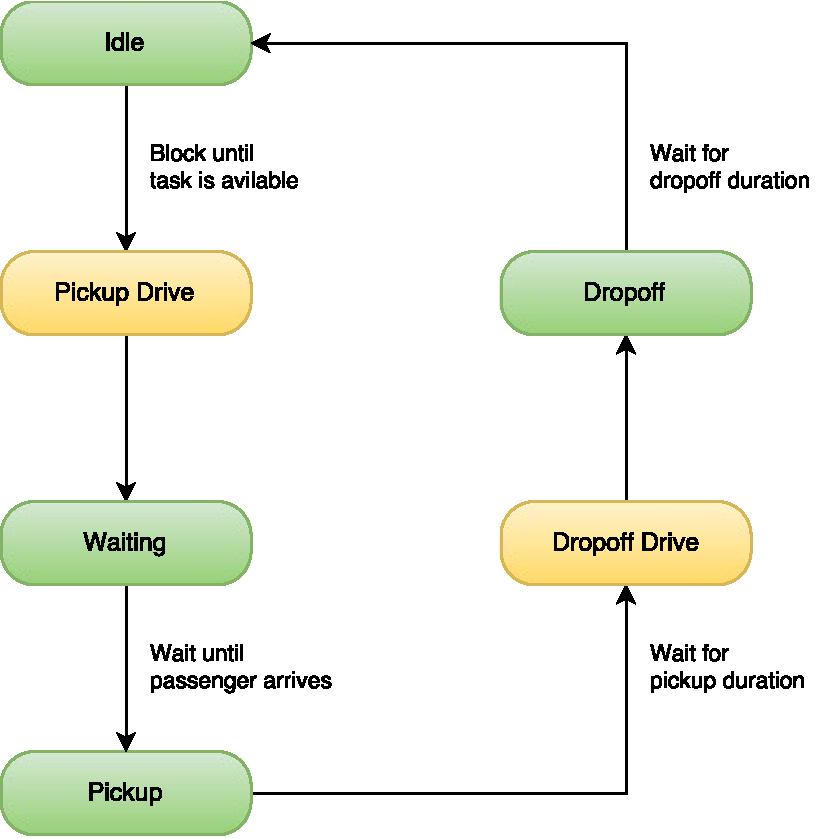
\includegraphics[width=0.7\textwidth]{figures/avstates.pdf}
    \caption{State chart of an AV agent. Activity states are displyed in green, while Leg states are yellow.}
    \label{fig:avstates}
\end{figure}

\subsection{Dispatcher Algorithm}

The dynamic dispatching of taxi vehicles is quite a complex scheduling problem,
which is quite hard to solve or needs numerous asumptions to be feasible. In
general, the problem will be a NP hard and heuristical solution strategies need
to be applied if fast solutions are needed. An overview, as well as a proposed
heuristic algorithm can be found in \citet{Maciejewski2015, Bischoff2016}.

The algorithm can be described in two different states:

\begin{description}
\item[Oversupply] occurs when there are more available autonomous vehicles than
requests. This means that each request can be assigned without delay. In that case,
as soon as a request arrives at the dispatcher, the closest vehicle to this request
is searched and assigned to serve the customer.
\item[Undersupply] is the case when all autonomous vehicles are occupied. In that
case requests will stack up, which cannot be handled immediately. In this case the
algorithm works the other way round: As soon as an autonomous vehicle gets available,
it is dispatched to the closest request.
\end{description}

According to the beforementioned papers this strategy gives a near-optimal solution,
although providing fast computational times.

The implementation for this thesis is based on a spatial relaxation of the traffic
network. This means that a grid with a specific resolution in x and y is fitted
over the links. One of these grids saves the locations of all the available AVs,
while another grid saves the locations of all open requests. Because the grids have
a fixed structure, finding the closest AV or request is quite simple, since each
position in x and y belongs to one specific cell of the grid. If no option is found
in a certain cell, the search continues with all cells in its Moore neighborhood
(all 8 surrounding cells). If this still gives no result, the radius is increased
and so forth. When specifiying ``find at least $K$ hits'' as a stop criterion for
a search this resembles an approximate K-nearest-neighbor search based on a $L_1$
norm due to the grid character.
The procedure is depictred in \cref{fig:gridsearch}.

\begin{figure}
    \centering
    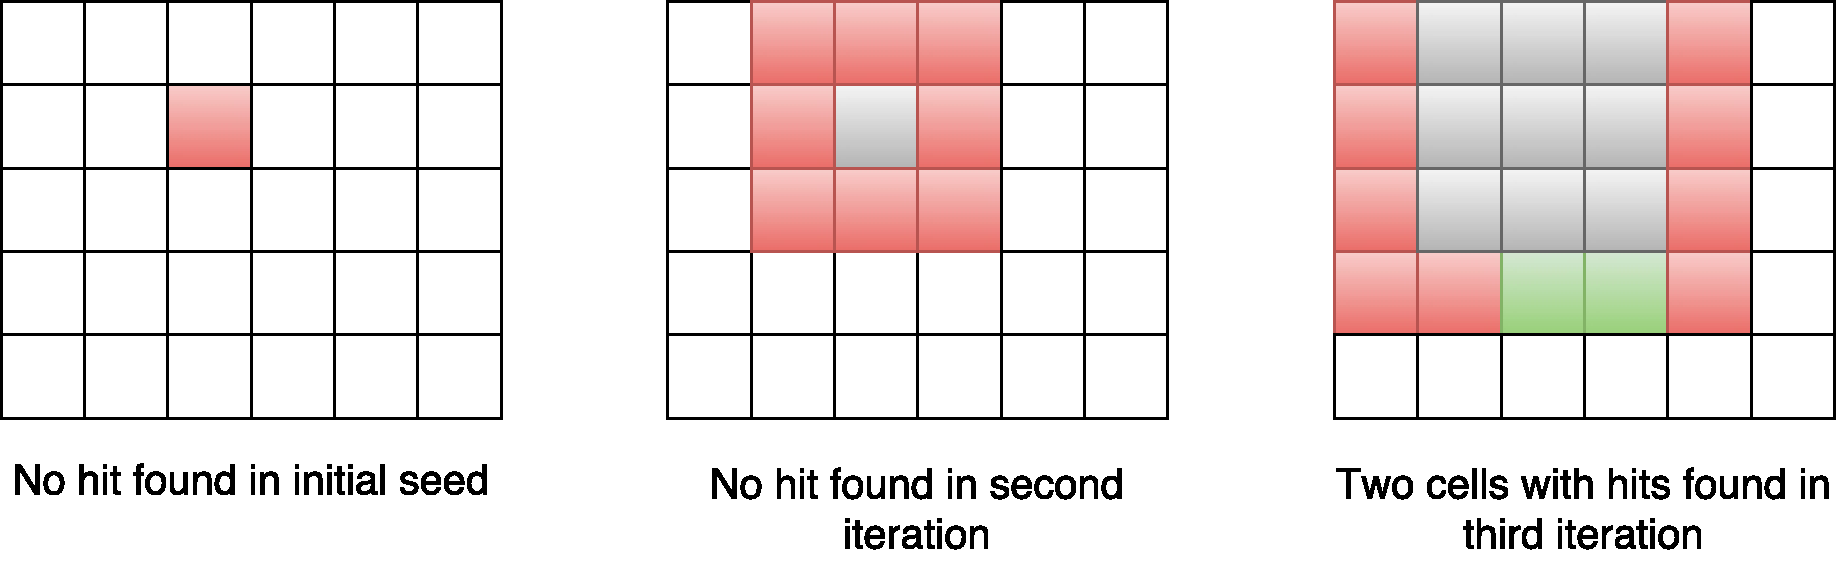
\includegraphics[width=1.0\textwidth]{figures/gridsearch.pdf}
    \caption{Schematic grid search algorithm for the dispatcher}
    \label{fig:gridsearch}
\end{figure}

This search algorithm imposes new parameters to the implementation, which basically
are the cell counts in horizontal and vertical direction. Depending on the topology
of the network, different parameters might be more efficient. If the grid is chosen
to be too dense, many iterations are needed in the algorithm, while a too sparse one
in the extreme case can lead to finding most of the items in only single cell.

In fact, for some topologies it might probably be more efficient to use different
data structures like a binary tree or quadtree to improve the search procedure.
Also more elaborate network search algorithms could be used, which make direct use
of the topology. \todo{cite example maybe}

\todo{Explain how this has been parallelized! Show spoeed improvement!}

For the Sioux Falls scenario it has been tested which impact the choice of the grid
size has on the results. I \cref{fig:gridsize} one can see that very high resolution
grids ($n=200$) lead to a great increase in computational time, due to the necessary
``expansion'' of unoccupied cells, as described above. On the contrary, very low
grid sizes lead to very poor results in terms of the overal average travel time of
the agents, because just selecting a random agent from one of a few cells is basically
just random assignment. A good value for the Sioux Falls network has been found to
be $n=20$, which is computed fastest over the whole range of shares and furthermore
does a good job in decreasing the overall travel time.

\begin{figure}
    \centering
    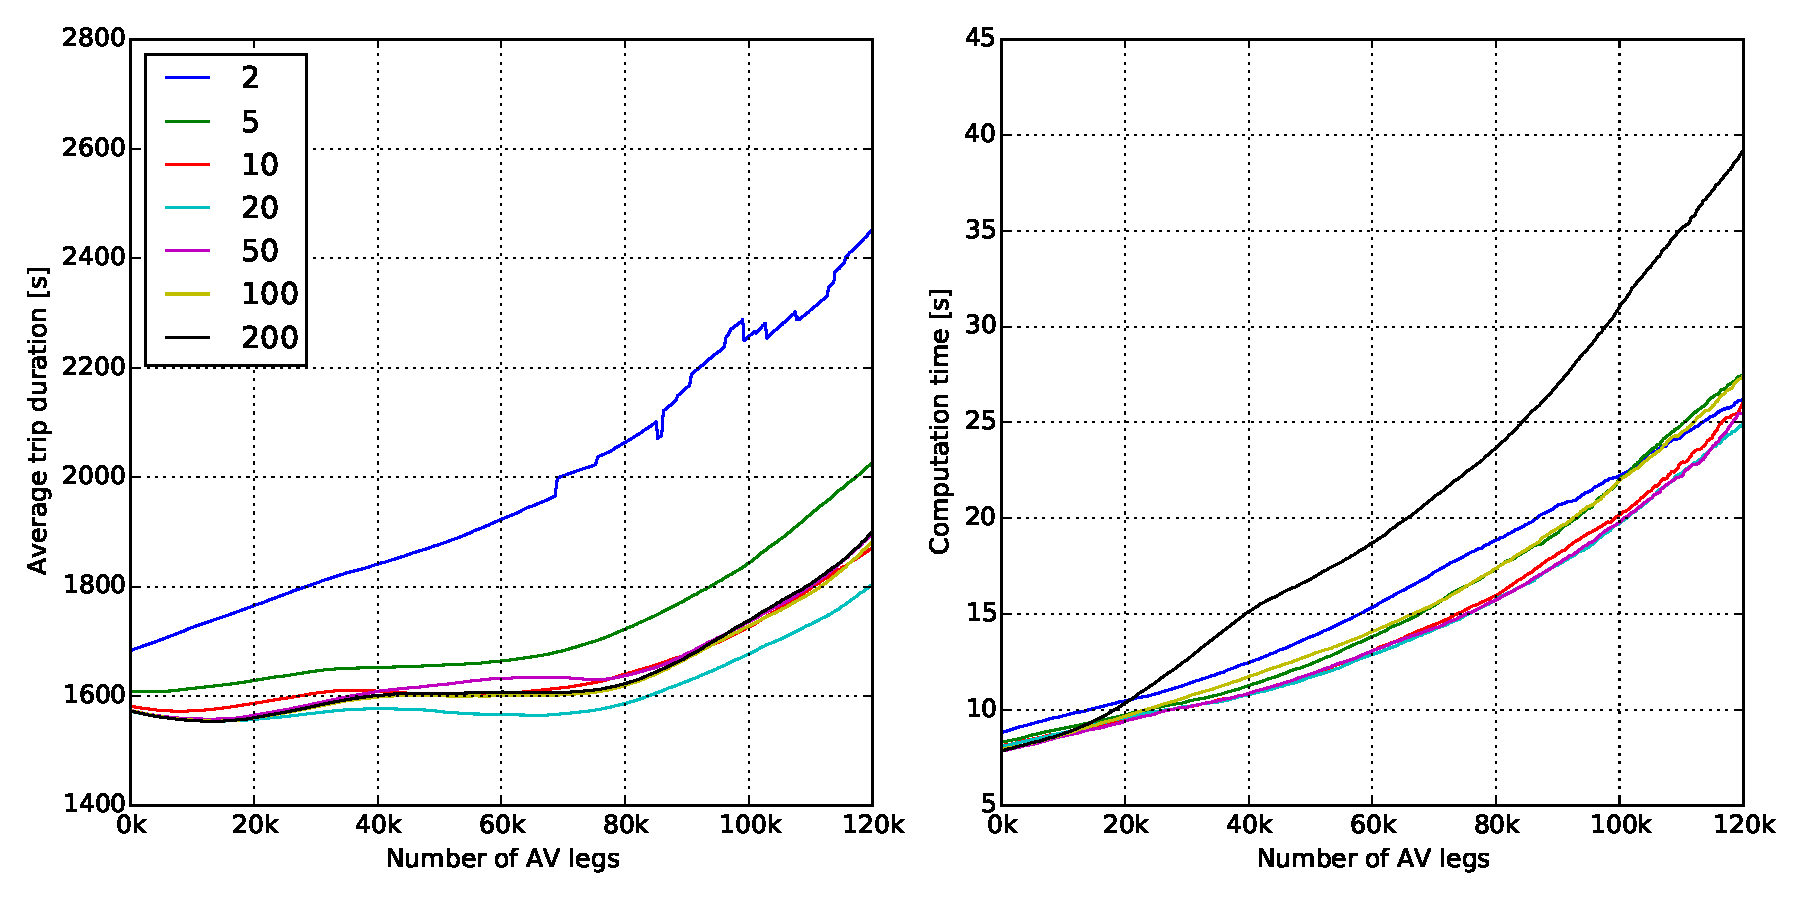
\includegraphics[width=1.0\textwidth]{figures/gridsize.pdf}
    \caption{Performance of different grid sizes in the dispatching algorithm for Sioux Falls}
    \label{fig:gridsize}
\end{figure}

\subsection{Distribution Algorithm}

At the beginning of a day simulation MATSim all the $n$ available AVs must be placed
somewhere in the network. Two simple distribution algorithms have been implemented
for the purpose of testing in this thesis.

The first one is \textbf{Random Distribution}. Here $n$ links are chosen randomly
from all available network links. While this is an easy distribution strategy for testing,
it create a quite unrealistic scenario. Obviously, in a real AV service, vehicles
would be relcoated over night, such that they can serve as many passengers as
possible during the morning peek.

Therefore a more elaborate distribution strategy has been implemented, which should
lead to more realistic results. Basically one can define a density over the network,
such that every link has a certain probability to get an AV assigned. Then, in $n$
steps, the $n$ available AVs are added to a link dependent on the assignment
probability.

This probability density can be based on many factors. The ones that are implemented
for this thesis are:

\begin{description}
\item[Population density] What is measured here is the population density in terms of
how many people are havingtheir ``home'' activity on a certain link.
\item[AV commuter density] Here for each link it is counted how many people will
have chosen the AV mode for their first leg, i.e. the one that is starting from home.
\end{description}

While the prior one is static, the latter on is dynamic in the sense that for every
iteration in the evolutionary learning, the density will change. So while the
population-density based distribution is a fixed constraint, the latter one captures
the factor of availability. For instance, if there are many agents using AVs in a
certain area, the availability is very high, and thus more people might be inclined
to use it. On the other hand, if availability is low in an area, it might lead to
longer waiting times and people are less likely to use AVs.

While it might be interesting to observe different patterns of availability,
for the first testing purposes the population density is better suited, since a
detailed investigation would need to be done if any results from the AV leg density
come from the mode choice of the agents or of feedback behaviour within the algorithm
itself.
